\section{Приклади}

\subsection{Перша породжувальна модель обличчя}

У 1972 році Фредерік Парке опубліковав статтю,
де було описано тривимірну модель обличчя \cite{Parke:1972}.
Вона містила лише 250 полігонів та 400 вершин,
проте могла імітувати різні людські емоції.

Модель з певним виразом обличчя створювалася за допомогою
двох фотографій асистента: одне збоку і одне фронтальне.
На обличчя асистента заздалегіть було нанесено необхідні полігони
(рис. \ref{fig:parke:face-paint}).
\begin{figure}[h]
  \centering
    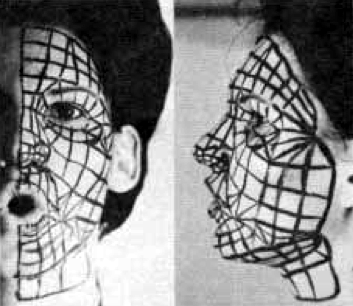
\includegraphics[width=0.5\textwidth]{images/Parke-face-paint}
  \caption{Пара ортогональних фотографій асистента з нанесеними полігонами}
  \label{fig:parke:face-paint}
\end{figure}

Найпершою роботою зі створення
тривимірної породжувальної моделі обличчя важається
дисертація Фредеріка Парке 1974 року \cite{Parke:1974}.
Ця модель могла імітувати не тільки різні емоції,
але й артикуляцію і різну форму обличчя
(рис. \ref{fig:parke:face-models}).
\begin{figure}[h]
  \centering
    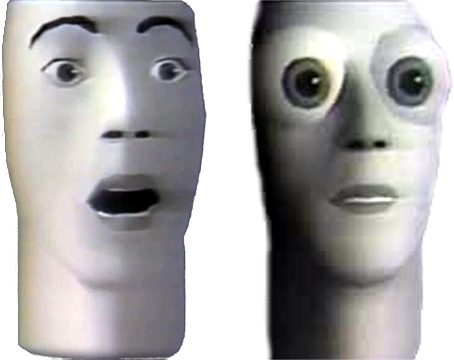
\includegraphics[width=0.5\textwidth]{images/Parke-faces}
  \caption{Моделі з різною формою очей та виразами облич}
  \label{fig:parke:face-models}
\end{figure}

Щоб оцінити приголомшливість цих результатів, пропоную згадати,
коли з'явилися перші тривимірні відеоігри,
персонажі яких мають анімовані об'ємні обличчя,
а не лише анімовану текстуру на голові.
Це не було можливо навіть у легендарній грі Quake,
що вийшла у 1996 році, хоча технологія існувала вже понад 20 років.

\subsection{Модель Базелівського університету}

У даній роботі використовується породжувальна модель обличчя
3D Basel Face Model (BFM)
розроблена командою Базельського університету
\cite{bfm09}.
Перший підхід,
яких дозволяє отримати тривимірну модель обличчя лише за одним фото,
було запропоновано Томасом Феттером та Фолькером Бланцом
\cite{blanz:vetter:1999}.
Вони використовували BFM та стохастичний градієнтний спуск \cite{sgd:1998},
що дозволяло досягти добрих результатів за 40 хвилин з процесором
Pentium III, 800MHz \cite{blanz:romdhani:vetter}.
У статті продемонстровано результат реконструкції
обличчя Тома Хенкса (рис. \ref{fig:bfm:tom-hanks})
за допомогою одного кадру з кінофільму ``Форрест Гамп''
(рис. \ref{fig:bfm:forrest-gump}).
\begin{figure}[h]
  \centering
  \begin{subfigure}[b]{0.3\textwidth}
    \centering
    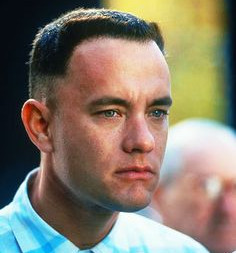
\includegraphics[width=\textwidth]{images/forrest-gump}
    \caption{Кадр з кінофільму ``Форрест Гамп''}
    \label{fig:bfm:forrest-gump}
  \end{subfigure}
  \begin{subfigure}[b]{0.3\textwidth}
    \centering
    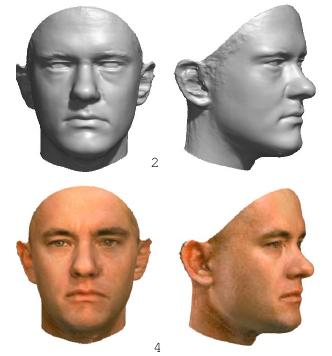
\includegraphics[width=\textwidth]{images/forrest-gump-model}
    \caption{Реконструкція голови Тома Хенкса}
    \label{fig:bfm:tom-hanks}
  \end{subfigure}
  \caption{Демонстрація роботи алгоритму дослідників з Базелівського університету}
\end{figure}

Згодом ті ж автори розробили та використали у своїй роботі
стохастичний алгоритм Ньютона \cite{blanz:vetter:2003},
яким досягли реконструкції просторової конфігурації обличчя за 4.5 хвилини на
Pentium 4, 2GHz.

Важливою деталлю цієї породжуючої моделі є те,
що кожна вершина різних моделей має однакове семантичне значення.
Краї очей, рота, кінчик носу, підборіддя та інші точки
знаходяться в однакових комірках масивів вершин моделей.
BFM розмічена опорними точками з наборів Farkas та MPEG4 FDP
(рис. \ref{fig:problems:feature-points}).
Відповідність точок дає змогу створювати власні множини опорних точок.
\begin{figure}[h]
  \centering
    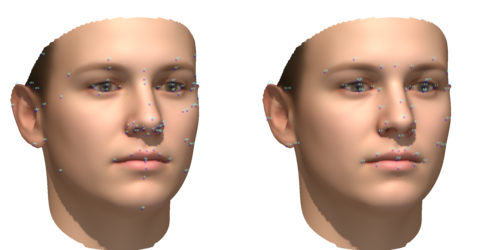
\includegraphics[width=\textwidth]{images/feature-points}
  \caption{Усереднені моделі облич з відміченими опорними точками}
  \label{fig:problems:feature-points}
\end{figure}

\subsection{Вітчизняна робота}

У 2011 році Максим Тищенко,
випускник Національного Технічного Университету України
``Київський Політехнічний Інститут'',
працюючи у Міжнародному науково-навчальному центрі
інформаційних технологій та систем над кандидатською дисертацією,
запропонував та запатентував
свій метод створення генеративної моделі обличчя та відновлення
тривимірної поверхні обличчя за одним або кількома фото \cite{tyshchenko:2011}.
Основні відмінності полягають у тому,
що задачу співставлення відповідних точок різних моделей
було представлено та розв'язано як супермодулярну
задачу розмітки \cite{Lovasz1983},
а нові моделі облич генеруються як зважене середнє.
Проте було наявне спрощення: самозатінення не бралося до уваги,
що дозволяло дуже швидко знаходити оптимальне освітлення
за пласкою моделлю затінення методом найменших квадратів.

\subsection{Сучасні роботи}

На момент написання дисертації одними з новітніх робот,
де було використано модель Базельського університету,
є методи відстеження обличчя \cite{Saito2016}
та переносу виразу обличчя однієї людини іншій \cite{thies2016face}.
Докладніше про них буде сказано в наступному підрозділі.
Останньою відомою роботою
є Large Scale 3D Morphable Models \cite{Booth:2017}~---~це
генеративна модель обличчя, яка отримана з тривимірних знімків $10$ тисяч людей
різної статі, віку та раси, що робить її дуже різноманітною та корисною
(рис.~\ref{fig:problems:lsfm}).

\begin{figure}[h]
  \centering
    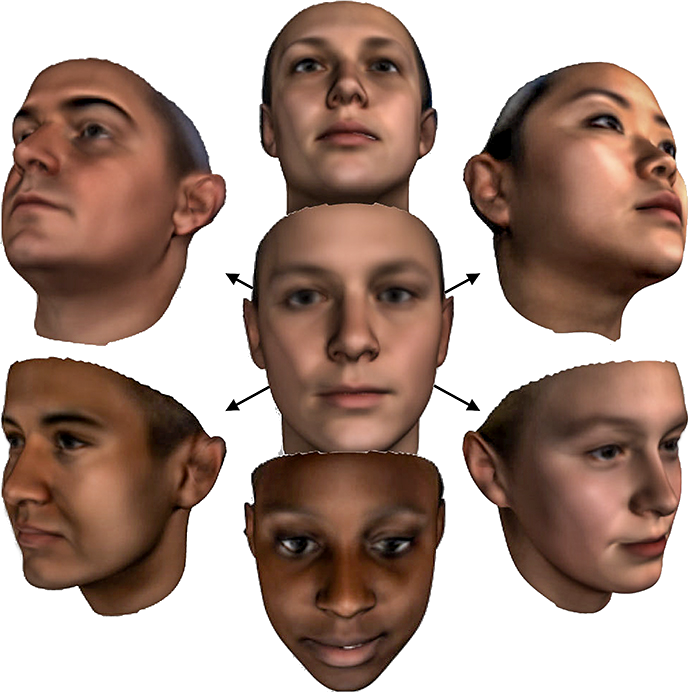
\includegraphics[width=0.5\textwidth]{images/lsfm}
  \caption{Приклади облич, що побудовані за допомогою LSFM}
  \label{fig:problems:lsfm}
\end{figure}
